\section{A Review of Differential Geometry}
The foundation of minimal surface theory comes from Differential Geometry so we will spend some time giving a brief overview of the key points. Further detail can be found in \cite{DoC} and \cite{EDG}.

\subsection{Gauss Map}
Given a surface M, at each point $p \in M$ there exists a tangent plane $T_pM$ and so we can define a unit normal at point $p$. Assuming M is an orientatable surface this unit normal $\mathbf N$ varies smoothly with $p$.

We can then define the Gauss Map, $G$ as a map from our surface M to the unit 2-sphere
$\mathit S^2 \subset \mathbb{R}^3$. Therefore it is the map $G:M \to \mathit S^2$ given by

\begin{displaymath}
\mathbf G(p) = \mathbf N_p =  \frac{(\mathbf X_u \times \mathbf X_v)}{|\mathbf X_u \times \mathbf X_v|}
\end{displaymath}

\subsection{First Fundamental Form}

This is a construct that allows us to measure lengths, angles and areas on a surface.

Let $\mathbf \alpha(t)= \mathbf X(u(t),v(t))$ be a curve in a surface $\mathbf X$, then its arc-length measured from a point $\alpha(t_0)$ is given by

\begin{displaymath}
\int_{t_0}^t ||\mathbf{\dot{\alpha}}(t)|| dt
\end{displaymath}

Take $\mathbf \alpha(t) = <X_1(u(t),v(t)),X_2(u(t),v(t)),X_3(u(t),v(t))>$ and using the chain rule:

\begin{eqnarray}
\nonumber
\mathbf{\dot{\alpha}}(t) &=& <\frac{\partial X_1}{\partial t},\frac{\partial X_2}{\partial t},\frac{\partial X_3}{\partial t}> \\
\nonumber
&=& <\frac{\partial X_1}{\partial u}\frac{\partial u}{\partial t}+ \frac{\partial X_1}{\partial v}\frac{\partial v}{\partial t},\frac{\partial X_2}{\partial u}\frac{\partial u}{\partial t}+ \frac{\partial X_2}{\partial v}\frac{\partial v}{\partial t},\frac{\partial X_3}{\partial u}\frac{\partial u}{\partial t}+ \frac{\partial X_3}{\partial v}\frac{\partial v}{\partial t}> \\
\nonumber
&=&\mathbf X_u \dot u+ \mathbf X_v \dot v
\end{eqnarray}

Then 
\begin{eqnarray}
\nonumber
||\mathbf{\dot{\alpha}}||^2 &=& (\mathbf X_u \dot u+ \mathbf X_v \dot v) \cdot (\mathbf X_u \dot u+ \mathbf X_v \dot v) \\
\nonumber
&=&(\mathbf X_u \cdot \mathbf X_u)\dot{u}^2 +(\mathbf X_u \cdot \mathbf X_v)\dot{u}\dot{v} + (\mathbf X_v \cdot \mathbf X_u)\dot{v}\dot{u} + (\mathbf X_v \mathbf X_v)\dot{v}^2 \\
\nonumber
&=&(\mathbf X_u \cdot \mathbf X_u)\dot{u}^2 + 2(\mathbf X_u \cdot \mathbf X_v)\dot{u}\dot{v} + (\mathbf X_v \mathbf X_v)\dot{v}^2 \\
\nonumber
&=& E\dot{u}^2 + 2F\dot{u}\dot{v} + G\dot{v}^2
\end{eqnarray}

Where we define the coefficients E, F and G as:

\begin{displaymath}
E = \mathbf X_{u} \cdot \mathbf X_u
\end{displaymath}

\begin{displaymath}
F = \mathbf X_{u} \cdot \mathbf X_v
\end{displaymath}

\begin{displaymath}
G = \mathbf X_{v} \cdot \mathbf X_v
\end{displaymath}


\subsection{Second Fundamental Form}
We take a surface S parametrised by $\mathbf x(u,v)$, a point p $\in S$ and a parametrised curve on S, $\alpha (t) = \mathbf x(u(t),v(t))$. (In order to keep the notation simple all functions that appear below denote their values at the point $p$).

Now the tangent vector to $\alpha (t)$ at p is 
\begin{displaymath}
\alpha ' = \mathbf x_u du+ \mathbf x_v dv
\end{displaymath}
and 
\begin{displaymath}
d\mathbf N(\alpha ')=\mathbf N'(u(t),v(t))=\mathbf N_udu+\mathbf N_vdv
\end{displaymath}

The second fundamental form in the basis $\{ \mathbf x_u, \mathbf x_v \}$ is given by

\begin{displaymath}
II_p = <d\mathbf N(\alpha'),\alpha'> 
\end{displaymath}

\begin{displaymath}
= -<(\mathbf N_u du + \mathbf N_v dv ) , ( \mathbf x_u du+ \mathbf x_v dv) >
\end{displaymath}

\begin{displaymath}
= -<\mathbf N_u, \mathbf x_u> du^2 - 2<\mathbf N_v, \mathbf x_u>du dv -<\mathbf N_v, \mathbf x_v> dv^2
\end{displaymath}

\begin{displaymath}
= <\mathbf N, \mathbf x_{uu}>(du)^2 + 2<\mathbf N, \mathbf x_{uv}>du dv + <\mathbf N, \mathbf x_{vv}> dv^2
\end{displaymath}

Generally we write this as

\begin{displaymath}
L du^2 + M du dv + N dv^2
\end{displaymath}

Where we define the coefficients L, M and N as:

\begin{displaymath}
L = \mathbf x_{uu} \cdot \mathbf N
\end{displaymath}

\begin{displaymath}
M = \mathbf x_{uv} \cdot \mathbf N
\end{displaymath}

\begin{displaymath}
N = \mathbf x_{vv} \cdot \mathbf N
\end{displaymath}

\subsection{Gaussian and Mean Curvature}
\label{MeanCurve}
The Gaussian and Mean Curvature, K and H measure the rate of change of the Gauss Map.

Given a surface $\mathbf{X}(u,v)$ with Guass Map $\mathbf{G}(p) = \mathbf N_p$ then

\begin{eqnarray}
\nonumber
K &=& \det(-d\mathbf N_p) = a_{11}a_{22} - a_{12}a_{21} \\
\nonumber
H &=& \frac{1}{2}\mbox{Trace}(-d\mathbf N_p) = \frac{1}{2}(a_{11}+ a_{22})
\end{eqnarray}

where 

\begin{displaymath}
d\mathbf N_p =
\left( \begin{array}{cc}
a_{11} & a_{21} \\
a_{12} & a_{22}
\end{array} \right)
\end{displaymath}

Such that
\begin{eqnarray}
\nonumber
\mathbf G_*(\mathbf x_u) &=& \mathbf N_u(p) = a_{11} \mathbf x_u + a_{21} \mathbf x_v \\
\nonumber
\mathbf G_*(\mathbf x_v) &=& \mathbf N_v(p) = a_{12} \mathbf x_u + a_{22} \mathbf x_v
\end{eqnarray}

These curvatures can also be expressed in terms of the principal curvatures of a surface. If you imagine a surface has two principal directions that span the surface (it being a 2 dimensional object) then these principal curvatures give the curvature along those curves. Taking these principal curvatures as $\kappa_1$ and $\kappa_2$ we get

\begin{displaymath}
K=\kappa_1\kappa_2
\end{displaymath}
\begin{displaymath}
H=\frac{1}{2}(\kappa_1+\kappa_2)
\end{displaymath}

The preceding definitions for Gauss and Mean curvature give the best idea of actually what the two curvatures are measuring. We will also meet $dN_p$ again later as the \emph{Weingarten Map}, A when we come to generalise minimal surfaces to higher dimensions.

We can however use Gauss's \emph{Theorema Egregium} to write these curvatures in terms of the first and second fundamental form. They are easiest to calculate in this form.

Giving

\begin{equation}
K = \frac{LN - M^2}{EG-F^2}
\label{equ:K}
\end{equation}

\begin{equation}
H = \frac{LG-2MF+NE}{2(EG-F^2)}
\label{equ:H}
\end{equation}


\newpage
\subsection{Examples}
As with much mathematics it's easiest to see the above ideas in the form of a couple of examples.
\begin{example}[Graph Type Parametrisation]
\label{Saddle}
For the saddle given by 

\begin{displaymath}
\mathbf x(u,v) = (u,v,u^2-v^2)
\end{displaymath}

\begin{figure}[htbp]
	\centering
       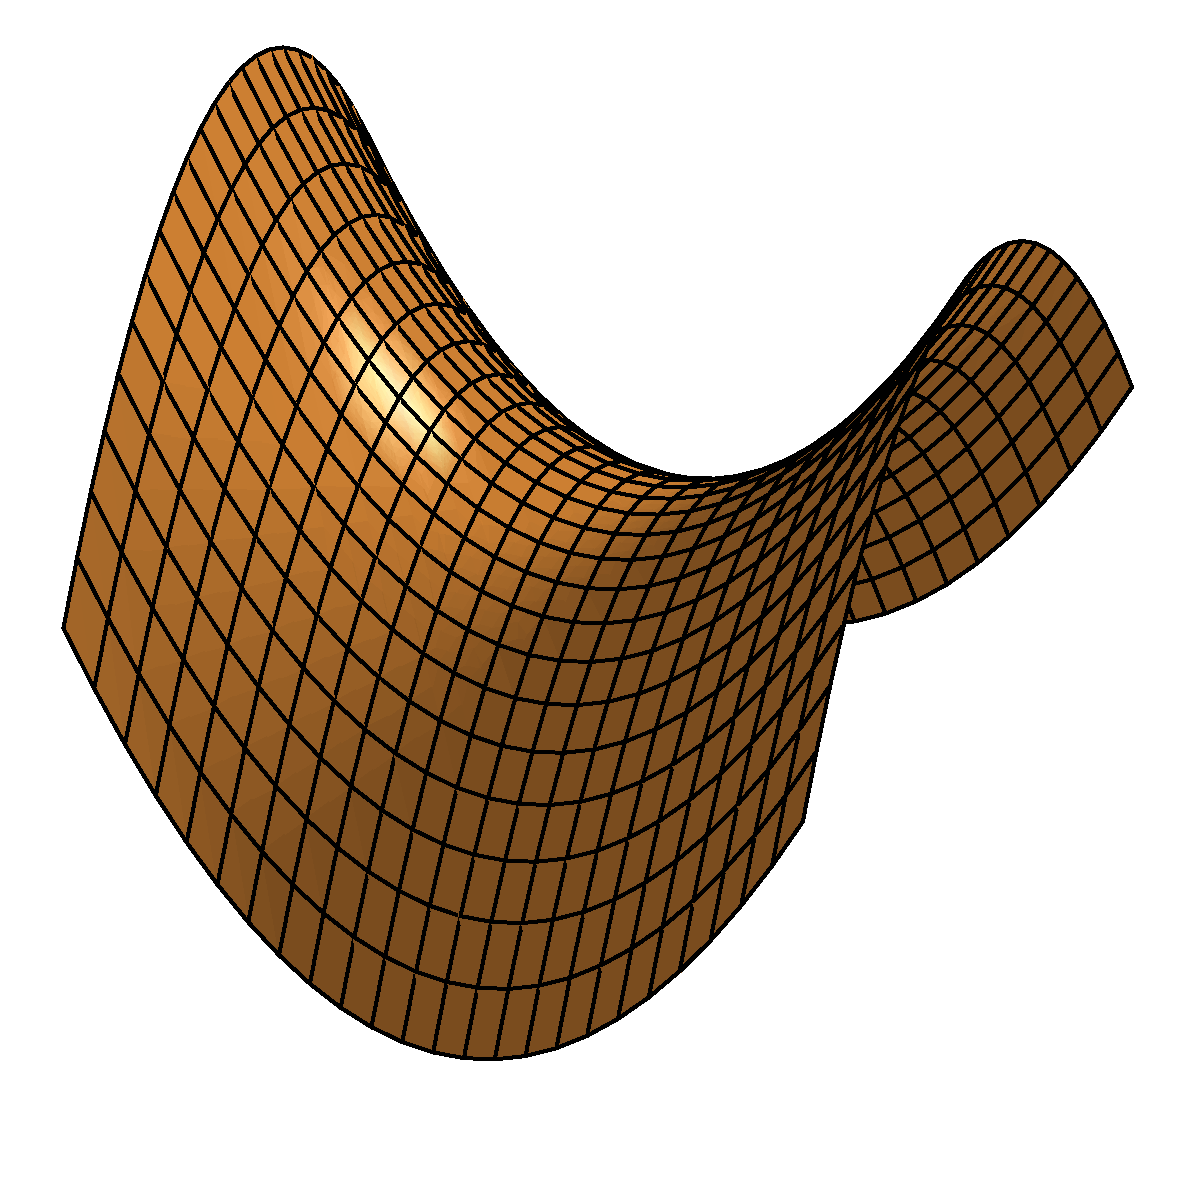
\includegraphics[width=8cm]{Images/Saddle.eps}
   \caption{Saddle}
   \label{fig:saddle}
\end{figure} 

Calculate the Gauss Map and the Second Fundamental Form. 

\begin{eqnarray}
\nonumber
\mathbf x_u &=& (1, 0 , 2u) \\
\nonumber
\mathbf x_v &=& (0, 1, -2v) \\
\nonumber
\mathbf x_{uu} &=& (0, 0 , 2) \\
\nonumber
\mathbf x_{vv} &=& (0, 0, -2) \\
\nonumber
\mathbf x_{uv} &=& (0, 0 , 0)
\end{eqnarray}

The Gauss map is then:
\begin{eqnarray}
\nonumber
G(p) = \mathbf N_p &=& \frac{(\mathbf x_u \times \mathbf x_v)}{|\mathbf x_u \times \mathbf x_v|} \\
\nonumber
&=&\frac{1}{\sqrt{1+4u^2+4v^2}}(-2u,2v,1)
\end{eqnarray}

The coefficients for the second fundamental form are:

\begin{eqnarray}
\nonumber
L &=& \mathbf x_{uu} \cdot \mathbf N = 2\,{\frac {1}{\sqrt {1+4\,{u}^{2}+4\,{v}^{2}}}}\\
\nonumber
M &=& \mathbf x_{uv} \cdot \mathbf N = 0\\
\nonumber
N &=& \mathbf x_{vv} \cdot \mathbf N = -2\,{\frac {1}{\sqrt {1+4\,{u}^{2}+4\,{v}^{2}}}}
\end{eqnarray}

So

\begin{displaymath}
II_p = ({\frac {1}{\sqrt {1+4\,{u}^{2}+4\,{v}^{2}}}})(2,0,-2)
\end{displaymath}

Then at the point p, $X(0,0)$ find the Gaussian and the Mean Curvature.

\begin{eqnarray}
\nonumber
\mathbf N_u &=& (-2,0,0) \\
\nonumber
\mathbf N_v &=& (0,2,0)
\end{eqnarray}

Projecting into the tangent plane gives

\begin{displaymath}
\mathbf N_u = -2 \mathbf x_u + 0 \mathbf x_v
\end{displaymath}

\begin{displaymath}
\mathbf N_v = 0 \mathbf x_u + 2 \mathbf x_v
\end{displaymath}

\begin{displaymath}
d\mathbf N_p =
\left( \begin{array}{cc}
-2 & 0 \\
0 & 2
\end{array} \right)
\end{displaymath}

So $ K(p) = 2 \cdot -2 = -4 $ and $H(p) = \frac{1}{2}(2 + -2) = 0$
\end{example}
\newpage

\begin{example}[Surface of Rotation]

For the surface formed by rotating $y=x^2$ about the y-axis calculate the Gauss Map and the Second Fundamental Form. 

\begin{figure}[htbp]
	\centering
       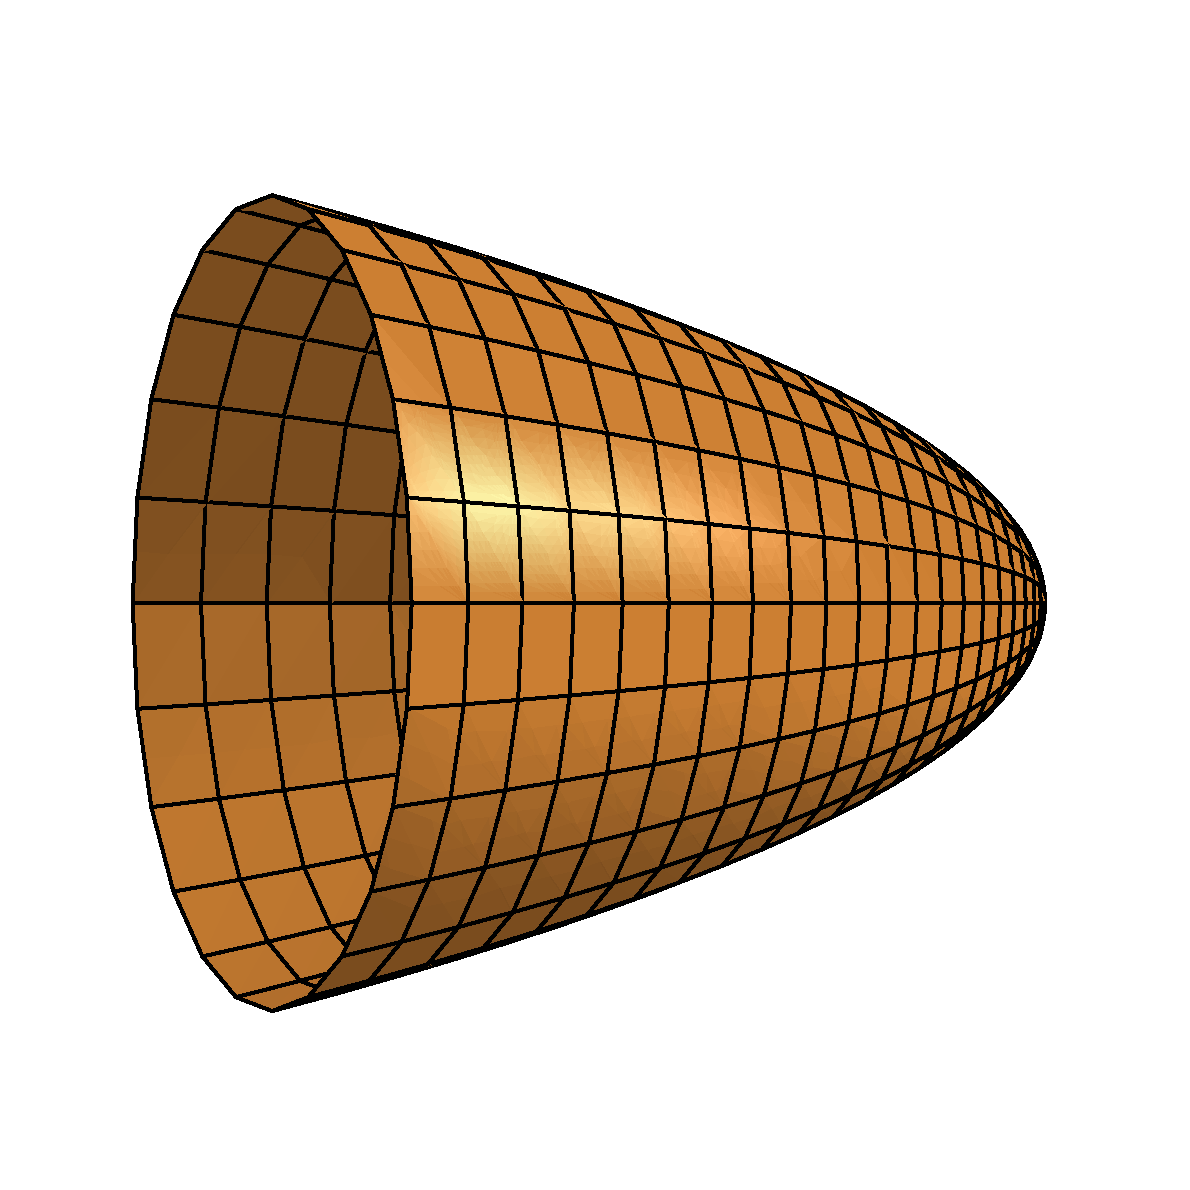
\includegraphics[width=8cm]{Images/Paraboloid.eps}
   \caption{Paraboloid}
   \label{fig:paraboloid}
\end{figure} 

Parametrised as $ \mathbf x(u,v) = (u\cos(v),u^2,u\sin(v))$

\begin{displaymath}
\mathbf x_u = (\cos v, 2u , \sin v) \, \,
\mathbf x_v = (-u \sin v, 0, u \cos v)
\end{displaymath}

\begin{displaymath}
\mathbf x_{uu} = (0, 2 , 0) \, \,
\mathbf x_{vv} = (- u \cos v, 0, - u  \sin v)
\end{displaymath}

\begin{displaymath}
\mathbf x_{uv} = (- \sin v, 0 , \cos v)
\end{displaymath}

The Gauss map is then:
\begin{eqnarray}
\nonumber
\mathbf G(p) &=& \frac{(\mathbf x_u \times \mathbf x_v)}{|\mathbf x_u \times \mathbf x_v|} \\ 
\nonumber
&=&\frac{1}{\sqrt{1+4u^2}}(2u cos v , -1 ,2u sin v)
\end{eqnarray}

The Second Fundamental Form is

\begin{displaymath}
II_p = \frac {-1}{\sqrt{1+4u^2}}(2,0, 2u^2)
\end{displaymath}

Then at the point p, $\mathbf x(\frac{1}{2},0)$ find the Gaussian and the Mean Curvature.

\begin{eqnarray}
\nonumber
\mathbf N_u &=& (\frac{1}{2}\sqrt{2},\frac{1}{2}\sqrt{2},0) = \frac{1}{2}\sqrt{2} \cdot \mathbf x_u + 0 \cdot \mathbf x_v \\
\nonumber
\mathbf N_v &=& (0,0,\frac{1}{2}\sqrt{2}) = 0 \cdot \mathbf x_u + \sqrt{2} \cdot \mathbf x_v
\end{eqnarray}

\begin{displaymath}
d\mathbf N_p =
\left( \begin{array}{cc}
\frac{1}{2}\sqrt{2} & 0 \\
0 & \sqrt{2}
\end{array} \right)
\end{displaymath}

So $ K = -\frac{1}{2}\sqrt{2} \cdot -\sqrt{2} = 1 $ and $H = \frac{1}{2}(-\frac{1}{2}\sqrt{2} - \sqrt{2}) = -\frac{3}{4}\sqrt{2}$

\end{example}

\subsection{What is a minimal surface?}
We now have enough differential geometry to define a minimal surface.

\begin{definition}[Minimal Surface]
A surface whose mean curvature, $H=0$ at all points. (E.g. note that the saddle in Example \ref{Saddle} is not minimal since although at $X(0,0)$, $H=0$ this is not the case elsewhere.)
\end{definition}
